% LaTeX Main Document for Sebastian Mayrhofers Final Thesis 
% created 1 August 2023
% by Sebastian Mayrhofer (may also be called basti-debug)



% Preamble (Angaben gelten für das ganze Dokument)
% Hilfe für Bibtex Einträge: https://www.literatur-generator.de
% ------------------------------------------------
% rote Umrandungen bei Verlinkungen entfernen: hidelinks
% 12pt als Standardschriftgröße
% A4-Dokument
% twoside (zweiseitiges Dokument): nur so werden verschiedene Fußzeilen für gerade bzw. ungerade Seitenzahlen übernommen
% article: Dokumentvorlage
\documentclass[hidelinks,12pt,a4paper,twoside]{article}
% Einbinden von Paketen
% ---------------------
\usepackage{titlesec} 						% ermöglicht die Verwendung der title- und section-Befehle
\usepackage[utf8]{inputenc}					% ermöglicht das Verwenden von Umlauten - linux od osx

\usepackage[top=3.5cm,left=3cm,right=2cm,bottom=2.5cm,headsep=0.3in,headheight=1in]{geometry} % Seitenränder
\usepackage{graphicx} 						% ermöglicht die Verwendung des includegraphics-Befehls zur Einbindung von Bildern
\usepackage{fancyhdr} 						% ermöglicht die einfache Erstellung von Kopf- und Fußzeilen
\usepackage{setspace} 						% ermöglicht Veränderung verschiedener Abstände
\usepackage{array} 							% ermöglicht unter anderem das Erstellen von benutzerdefinierten Vorlagen für Tabellenspalten
\usepackage[export]{adjustbox} 				% Umrandung von Bildern
\usepackage[nottoc,numbib]{tocbibind} 		% ermöglicht die Erstellung eines Inhaltsverzeichnisses
\usepackage{tocloft}
%\renewcommand\cftsecafterpnum{\vskip0pt}
%\usepackage{tocbasic}

\setlength{\cftsubsecnumwidth}{3em} 		% Set distance between number and text of subsection in table of contents

\makeatletter                               % definiert den Abstand zwischen Nummer und Beschriftung im Abb. u Tabellenverzeichnis
\renewcommand*\l@table{\@dottedtocline{1}{3em}{5em}}
\renewcommand*\l@figure{\@dottedtocline{1}{1.5em}{4em}}
\makeatother

\usepackage{color} 							% ermöglicht das Erstellen von benutzerdefinierten Farben

\usepackage{longtable}						% Unterstützung für mehrseitige Tabellen
\usepackage[ngerman]{babel}					% Deutsche Bezeichnungen 

\usepackage[backend=biber,citestyle=verbose, bibstyle=verbose]{biblatex} %mehrsprachiges Bibliotheks(Literatur-)verzeichnis
\usepackage[babel,german=guillemets]{csquotes} %deutsches Anführungszeichen
\addbibresource{bibliography.bib}

\usepackage{blindtext} 						% Blindtext
\usepackage{url} 							% Formatierung von URLs
\usepackage[bottom,hang,stable]{footmisc} 	% Fußnoten immer am unteren Ende der Seite
\usepackage{caption} 						% ermöglicht das Anpassen von diversen Beschriftungen
\usepackage{subcaption} 					% ermöglicht das Erstellen von Unterbezeichnungen (subfigures)
\usepackage{hyperref} 						% Hyperlinks im Dokument
\usepackage{pdfpages} 						% einbinden von PDF-Dateien
\usepackage{amsmath} 						% grundlegende mathematische Funktionen

\usepackage{listings,xcolor} 				% ermöglicht das Einbinden von Codesegmenten
\usepackage{listingsutf8} 					% ermöglicht das Einbinden von Codesegmenten

\usepackage{float} 							% Positionierung verschiedener Objekte
\usepackage{footnote} 						% ermöglicht das Anpassen von Fußnoten
\usepackage{enumitem} 						% ermöglicht das Anpassen von Aufzählungen
\usepackage{longtable} 						% erlaubt mehrseitige Tabellen
\usepackage{url} 							% gibt eine schöner formatierte Internetadresse aus
\usepackage{bold-extra}


% allgemein gültige Formateinstellungen
% -------------------------------------
\renewcommand{\familydefault}{\sfdefault} 	% set Font-Family to a similar font like Arial
\raggedbottom 								% Abschnitte werden nicht auseinander gezogen, um den restlichen Platz auf einer Seite zu füllen
%\raggedright 								% gesamtes Dokument linksbündig (auch Paragraphen) OHNE Silbentrennung

\usepackage{ragged2e}						% gesamtes Dokument linksbündig (auch Paragraphen) MIT Silbentrennung
\RaggedRight

\onehalfspacing 							% 1.5-facher Abstand zwischen den Zeilen

\renewcommand{\arraystretch}{1.05} 			% Vergrößerung des Abstands zwischen den Tabellenzeilen
\newcolumntype{C}[1]{>{\centering\arraybackslash}p{#1}} % erstellen eines Spaltentyps mit zentriertem Inhalt unter der Angabe einer Spaltenbreite
\newcolumntype{L}[1]{>{\raggedright\arraybackslash}p{#1}} % erstellen eines Spaltentyps mit linksbündigem Inhalt unter der Angabe einer Spaltenbreite

\setlength{\footnotemargin}{0.5cm} 			% Abstand zwischen Fußnotennummer und -text
\setlist{nosep} 							% zusätzliche Abstände bei Aufzählungen entfernen
\setlength{\parskip}{1em} 					% Abstand nach einem Absatz

% Abstände vor und nach Überschriften auf den verschiedenen Ebenen
\titlespacing\section       {0pt}{0pt plus 0pt minus 2pt}{0pt plus 2pt minus 2pt}
\titlespacing\subsection    {0pt}{0pt plus 0pt minus 2pt}{0pt plus 2pt minus 2pt}
\titlespacing\subsubsection {0pt}{0pt plus 0pt minus 2pt}{0pt plus 2pt minus 2pt}

% Formateinstellungen für Codesegmente
% ------------------------------------
\usepackage{caption}
\usepackage{minted} 						% für schöne Darstellung von Code
\usepackage{dingbat}						% für Sonderzeichen wie \carriagereturn

\setminted{
	autogobble,								% rückt Code soweit nach links wie möglich
	stepnumber=2,							% nur jede gerade Zeilennummer wird angezeigt
	fontfamily=tt,
	linenos=true,
	numberblanklines=true,
	numbersep=5pt,
	gobble=0,
	frame=single,
	framerule=0.4pt,
	framesep=2mm,
	funcnamehighlighting=true,
	tabsize=4,
	obeytabs=false,
	breaklines,
	breakafter=">/,
	breakbefore=. ,
	breaksymbolindentright=10pt,
	breaksymbolsepright=0pt
}

\newmintedfile[csharpcode]{csharp}{}
\newmintedfile[xamlcode]{xml}{}
\newmintedfile[bashcode]{bash}{}

\usepackage{etoolbox}
\AtBeginEnvironment{longlisting}{\dontdofcolorbox}
\def\dontdofcolorbox{\renewcommand\fcolorbox[4][]{##4}}		% zum Unterbinden des roten Rahmens im Quellcode um ein $-Zeichen

\newenvironment{longlisting}{\captionsetup{type=listing} \linespread{1.05}}{} % 1.05 facher Zeilenabstand bei listings

% Anlegen von benutzerdefinierten Farben für das Hervorheben bestimmter Teile des Codes
\definecolor{shblue}{rgb}{0.13,0.13,1} % Farbe für Schlüsselwörter
\definecolor{shgreen}{rgb}{0,0.5,0} % Farbe von Kommentaren
\definecolor{shred}{rgb}{0.9,0,0} % Farbe von Zeichenfolgen
\definecolor{lightgray}{gray}{0.95} % Hintergrundfarbe
\definecolor{maroon}{rgb}{0.5,0,0}
\definecolor{bg}{rgb}{0.95,0.99,0.99}

% benutzerdefiniertes Syntax-Highlighting für XAML
\lstdefinelanguage{XAML}
{
	morestring=[s]{"}{"},
	moredelim=[s][\color{black}]{>}{<},
	moredelim=[s][\color{maroon}]{<}{\ },
	moredelim=[s][\color{maroon}]{</}{>},
	moredelim=[l][\color{maroon}]{/>},
	moredelim=[l][\color{maroon}]{>},
	morecomment=[s]{<?}{?>},
	morecomment=[s]{<!--}{-->},
	commentstyle=\color{shgreen},
	stringstyle=\color{shblue},
	identifierstyle=\color{shred}
}

% spezifische Einstellungen für verschiedene Sprachen
\lstdefinestyle{csharp}
{
	language=[Sharp]C,
	commentstyle=\color{shgreen}, % Farbe für Kommentare
	keywordstyle=\color{shblue},
	stringstyle=\color{shred}
}

\lstdefinestyle{xaml}
{
	language=XAML
}

\skip\footins 30pt				% etwas größerer Abstand oberhalb Fußnote

% kapitelweise Nummerierung
\let\oldsection\section
\let\oldsubsection\subsection
\renewcommand{\section}{\counterwithin{figure}{section}\oldsection}
\renewcommand{\subsection}{\counterwithin{figure}{subsection}\oldsubsection}

\let\oldsectionL\section
\let\oldsubsectionL\subsection
\renewcommand{\section}{\counterwithin{listing}{section}\oldsectionL}
\renewcommand{\subsection}{\counterwithin{listing}{subsection}\oldsubsectionL}

\let\oldsectionT\section
\let\oldsubsectionT\subsection
\renewcommand{\section}{\counterwithin{table}{section}\oldsectionT}
\renewcommand{\subsection}{\counterwithin{table}{subsection}\oldsubsectionT}



% Anpassung diverser Beschriftungen
\captionsetup[listing] {labelfont=bf,textfont=it,format=hang,justification=raggedright}
\captionsetup[table]   {labelfont=bf,textfont=it,format=hang,justification=raggedright}
\captionsetup[figure]  {labelfont=bf,textfont=it,format=hang,justification=raggedright}

\captionsetup[figure]  {name=Abbildung} 		% Abbildungen
\captionsetup[table]   {name=Tabelle} 			% Tabellen
\captionsetup[longlisting]{name=Codeabschnitt}	% Codeabschnitte -> fkt. leider nicht


\newcommand{\cmd}[2]{\emph{#1}\space \textbf{#2}} % z.B.  \cmd{Get-Item}{C:\textbackslash temp\textbackslash test.txt}

\newcommand{\keyword}[1]{\texttt{\textbf{#1}}}	% für Code im Fließtext
  % Include Preamble File -> needed for all Settings of the Document 
\pagestyle{fancy}
% This Document is used for all reacuring Names 
% created by basti-debug
% 
% last change: 1 August 2023

\newcommand{\pjname}{ModTable}

\newcommand{\studentN}{Mayrhofer Sebastian}
\newcommand{\studentLastN}{Mayrhofer}
\newcommand{\studentSLN}{MayrhoferS}
\newcommand{\studentShort}{SM}

\newcommand{\supervisor}{Dipl.Ing. Rusch Helmut Elmar}

\newcommand{\PrintDate}{20.3.2023}

% HTL Header 

\lhead{\hspace{0.2cm} 
\includegraphics[height=1.04cm]{img/assets/htlr_logo.png}}
\chead{\textbf{HTBLuVA  Rankweil} 
	\\[0.05in]
	\footnotesize{\textit{Höhere Lehranstalt für Elektronik und Technische Informatik}}}
\rhead{
\includegraphics[height=1.04cm]{img/assets/htl_logo.jpg} \hspace{0.2cm}}

\fancyfoot{} 

\begin{document}
	\begin{center}
		\textbf {\huge {\uppercase {Diplomarbeit}}}
		\par \large {Gesamtprojekt}
		\par \textbf {\huge {\uppercase {\pjname}}}
		\vspace{0.3cm}
		\linebreak
		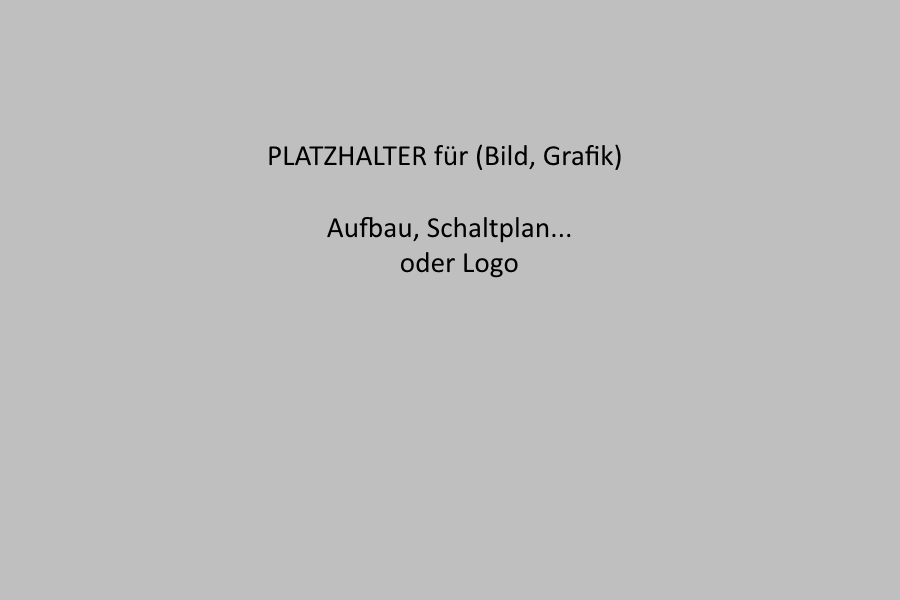
\includegraphics[frame, height=6cm]{img/assets/title_placeholder.png}
	\end{center}
	
	\vfill % damit der folgende am Blattende positioniert wird
	
	
	\begin{minipage}[t] {0.4\textwidth}
		\textbf{Team members:} \\
		\studentN \\
	\end{minipage}
	\begin{minipage}[t] {0.4\textwidth}
		\textbf{Supervisor:} \\		
		\supervisor \\
	\end{minipage}
	
	\par Rankweil, on the \PrintDate \\		
	
	\noindent\rule{\textwidth}{0.4pt}
	delivery note:
	\linebreak
	
	\begin{tabular}{p{7cm}C{6cm}}
		\hspace{1cm} DA original, on the \PrintDate & ........................................ \\ 
		& \supervisor \\ [2.5em]
		
		\hspace{1cm} DA digital, on the \PrintDate & ........................................ \\ 
		& \supervisor \\
	\end{tabular}
	
	
	% Empty Side
	\pagebreak
	\thispagestyle{empty}
	\cleardoublepage
	\pagebreak
	
	\SecAuth{\studentN} % festlegen der Verfasser dieses Kapitels
	
	\pagenumbering{Roman}
	\fancyfoot[LE,RO]{\thepage}
	\fancyfoot[LO,RE]{\DADate~\textbar~\pjname~\textbar ~\@SecAuth}
	\renewcommand{\footrulewidth}{0.4pt} % anzeigen Separator-Strich in der Fußzeile (standardmäßig deaktiviert)
	
	\section*{Declaration under oath}
I declare in lieu of an oath that I have written this thesis on my own and without any
without any help from others, that I have not used any sources or aids other than those indicated, and that
and that I have made the passages taken verbatim and in content from the sources used
as such.

\vspace{0.3cm}
\par Rankweil, on the \PrintDate
\linebreak
\linebreak

\begin{tabular}{p{7cm}C{5cm}}
	& ........................................ \\
	& \studentN  \\ [2.5em]
\end{tabular}


	
	
	
	
	\pagebreak
	
	\section*{Abbreviations \& Notes}
\begin{singlespace}	
	\begin{tabular}{ll}
		GUI    & Graphical User Interface \\
		OLED & Organic Light-Emitting Diode - \href{https://en.wikipedia.org/wiki/OLED}{Wikipedia article} \\
	\end{tabular}
\end{singlespace}
	
	\pagebreak
	
	\section{Concept design}
My final thesis, which i called \pjname, is a table which smartly adepts to the user.
Its aimed to fix the most annoying things with modern tables: cables, design and the function that everything just works. I want to fix this with my project, where i want to build one complete package where everything is well integrated and easy to use for the end user. This product is aimed at a work environment, ideally in a individual office. 

\subsection{Functions}
The Table should fulfill all basic functions of an office table so these are : 

\begin{enumerate}
\item A external Monitor 
\item Height adjustable Table
\item Camera System for Meetings
\item Microphone for Meetings
\vspace{0.3cm}

\textbf{And some additional features}

\item Status bar for notifications, timer, and calendar events
\begin{enumerate}
	\item Small OLED Screen for name of the event etc 
	\item LED Bar for Status indication (embedded into the table)
\end{enumerate}
\item Touch Screen inside the table for controlling all the functions
\end{enumerate}

\subsection{Milestones}
The Project will be worked through in 3 Stages (Versions)
\begin{enumerate}
	\item \textbf{Version 1}\\
	In the first prototype version the basic functionality should be created, so these following functions should be met: 
	\begin{enumerate}
		\item The screen should be able to adjust the table height
		\item The screen should be able to control all connected devices (Camera, Microphone)
		\item The connection from the table to the laptop should transmit the data for the Display and the connected Devices, and charge the device (Laptop)
	\end{enumerate}
	\item \textbf{Version 2}\\
	The second version should implement the aforementioned status bar, with the small OLED screen which should display the next calendar event or a timer, all of this should be controlled by the main control screen.
	
	\pagebreak
	 
	\item \textbf{Version 3}\\
	For the third version the table should be constructed an assembled, this milestone may be worked on parallel to the other versions so the sequence may not be correct. 
\end{enumerate}
	
	
	\pagebreak
	
	% Abbildungsverzeichnis
	% ---------------------
	% Abbildungsverzeichnis in Inhaltsverzeichnis
	\singlespacing % Zeilenabstand verringern
	\renewcommand{\listoffigures}{\begingroup
		\tocsection
		\tocfile{Abbildungsverzeichnis}{lof}
		\endgroup}
	\listoffigures % eigentlicher Befehl für das Anlegen des Abbildungsverzeichnisses
	\pagebreak
	
	% Tabellenverzeichnis
	% -------------------
	% Tabellenverzeichnis in Inhaltsverzeichnis
	
	\renewcommand{\listoftables}{\begingroup
		\tocsection
		\tocfile{Tabellenverzeichnis}{lot}
		\endgroup}
	
	\listoftables % eigentlicher Befehl für das Anlegen des Tabellenverzeichnisses
	\pagebreak
	
	% Codeabschnittsverzeichnis
	% -------------------------
	% Codeabschnittsverzeichnis in Inhaltsverzeichnis
	\stepcounter{section}		% increase section-counter
	\renewcommand{\listoflistingscaption}{\arabic{section}~~~Codeverzeichnis}
	\addcontentsline{toc}{section}{\arabic{section}~~~Codeverzeichnis} % Fügt Codevezeichnis ins Inhaltsverzeichnis ein
	
	\listoflistings
	\pagebreak
	
	% Quellenverzeichnis
	% ------------------
	%\onehalfspacing
	\printbibliography[heading=bibnumbered, title={Quellenverzeichnis}]
	
	\pagebreak
	
\end{document}
